\chapter{満足性評価のための指尖容積脈波によるストレス指標の提案}
\label{chap:pulsewave}

本章では,指尖容積脈波によるストレス指標と従来の評価手法の関連を把握するために行った実験について述べる.まず,提案する指標について述べた上で実験の内容と結果について述べる.

\section{ストレス指標}

\subsection{自律神経バランス(ANB)}

\subsection{最大リヤプノフ指数(LLE)}

\section{ストレス指標とヒューリスティック評価の関連性}

\subsection{実験方法と対象}

\begin{figure}[htbp]
  \begin{minipage}{0.5\hsize}
    \begin{center}
       \fbox{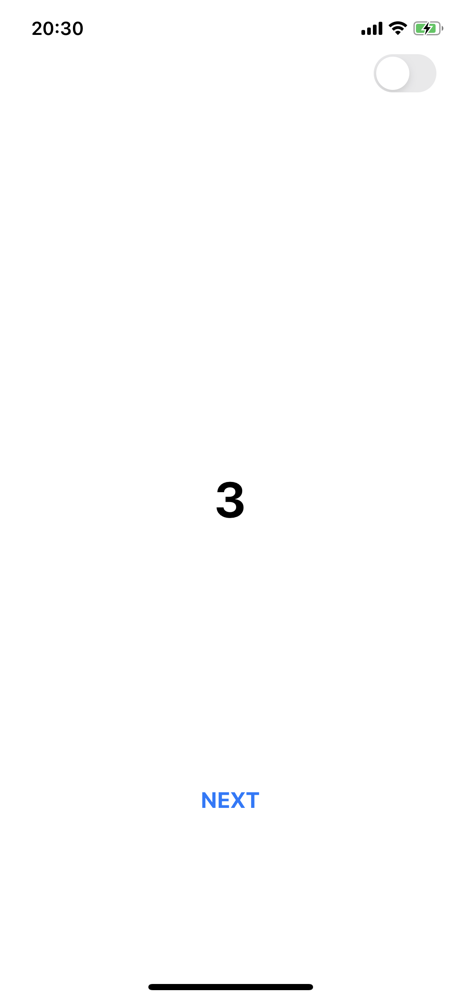
\includegraphics[width=40mm]{old1.png}}
    \end{center}
    \caption{実験マテリアル:数字の表示画面}
    \label{fig:lyspect}
  \end{minipage}
  \begin{minipage}{0.5\hsize}
    \begin{center}
       \fbox{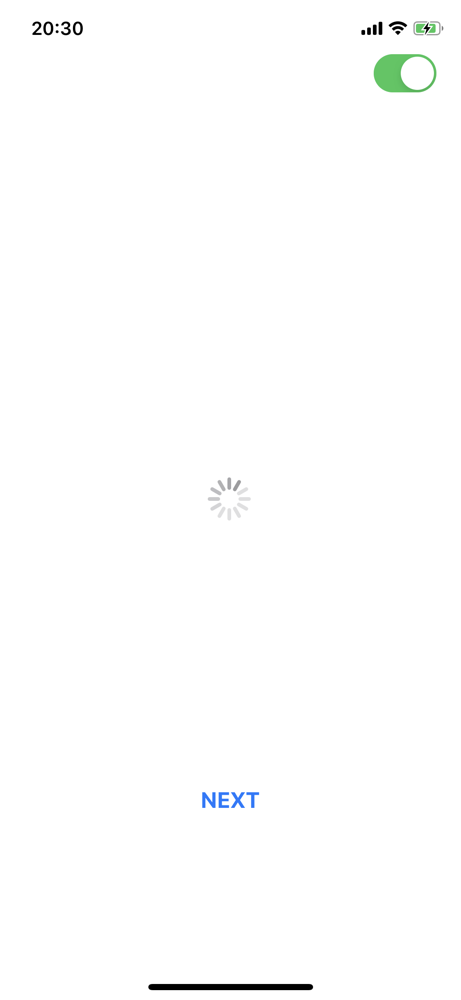
\includegraphics[width=40mm]{old2.png}}
    \end{center}
    \caption{実験マテリアル:数字の読込中画面}
    \label{fig:lyspect}
  \end{minipage}
\end{figure}

\begin{figure}[htbp]
  \begin{minipage}{\hsize}
    \begin{center}
       \fbox{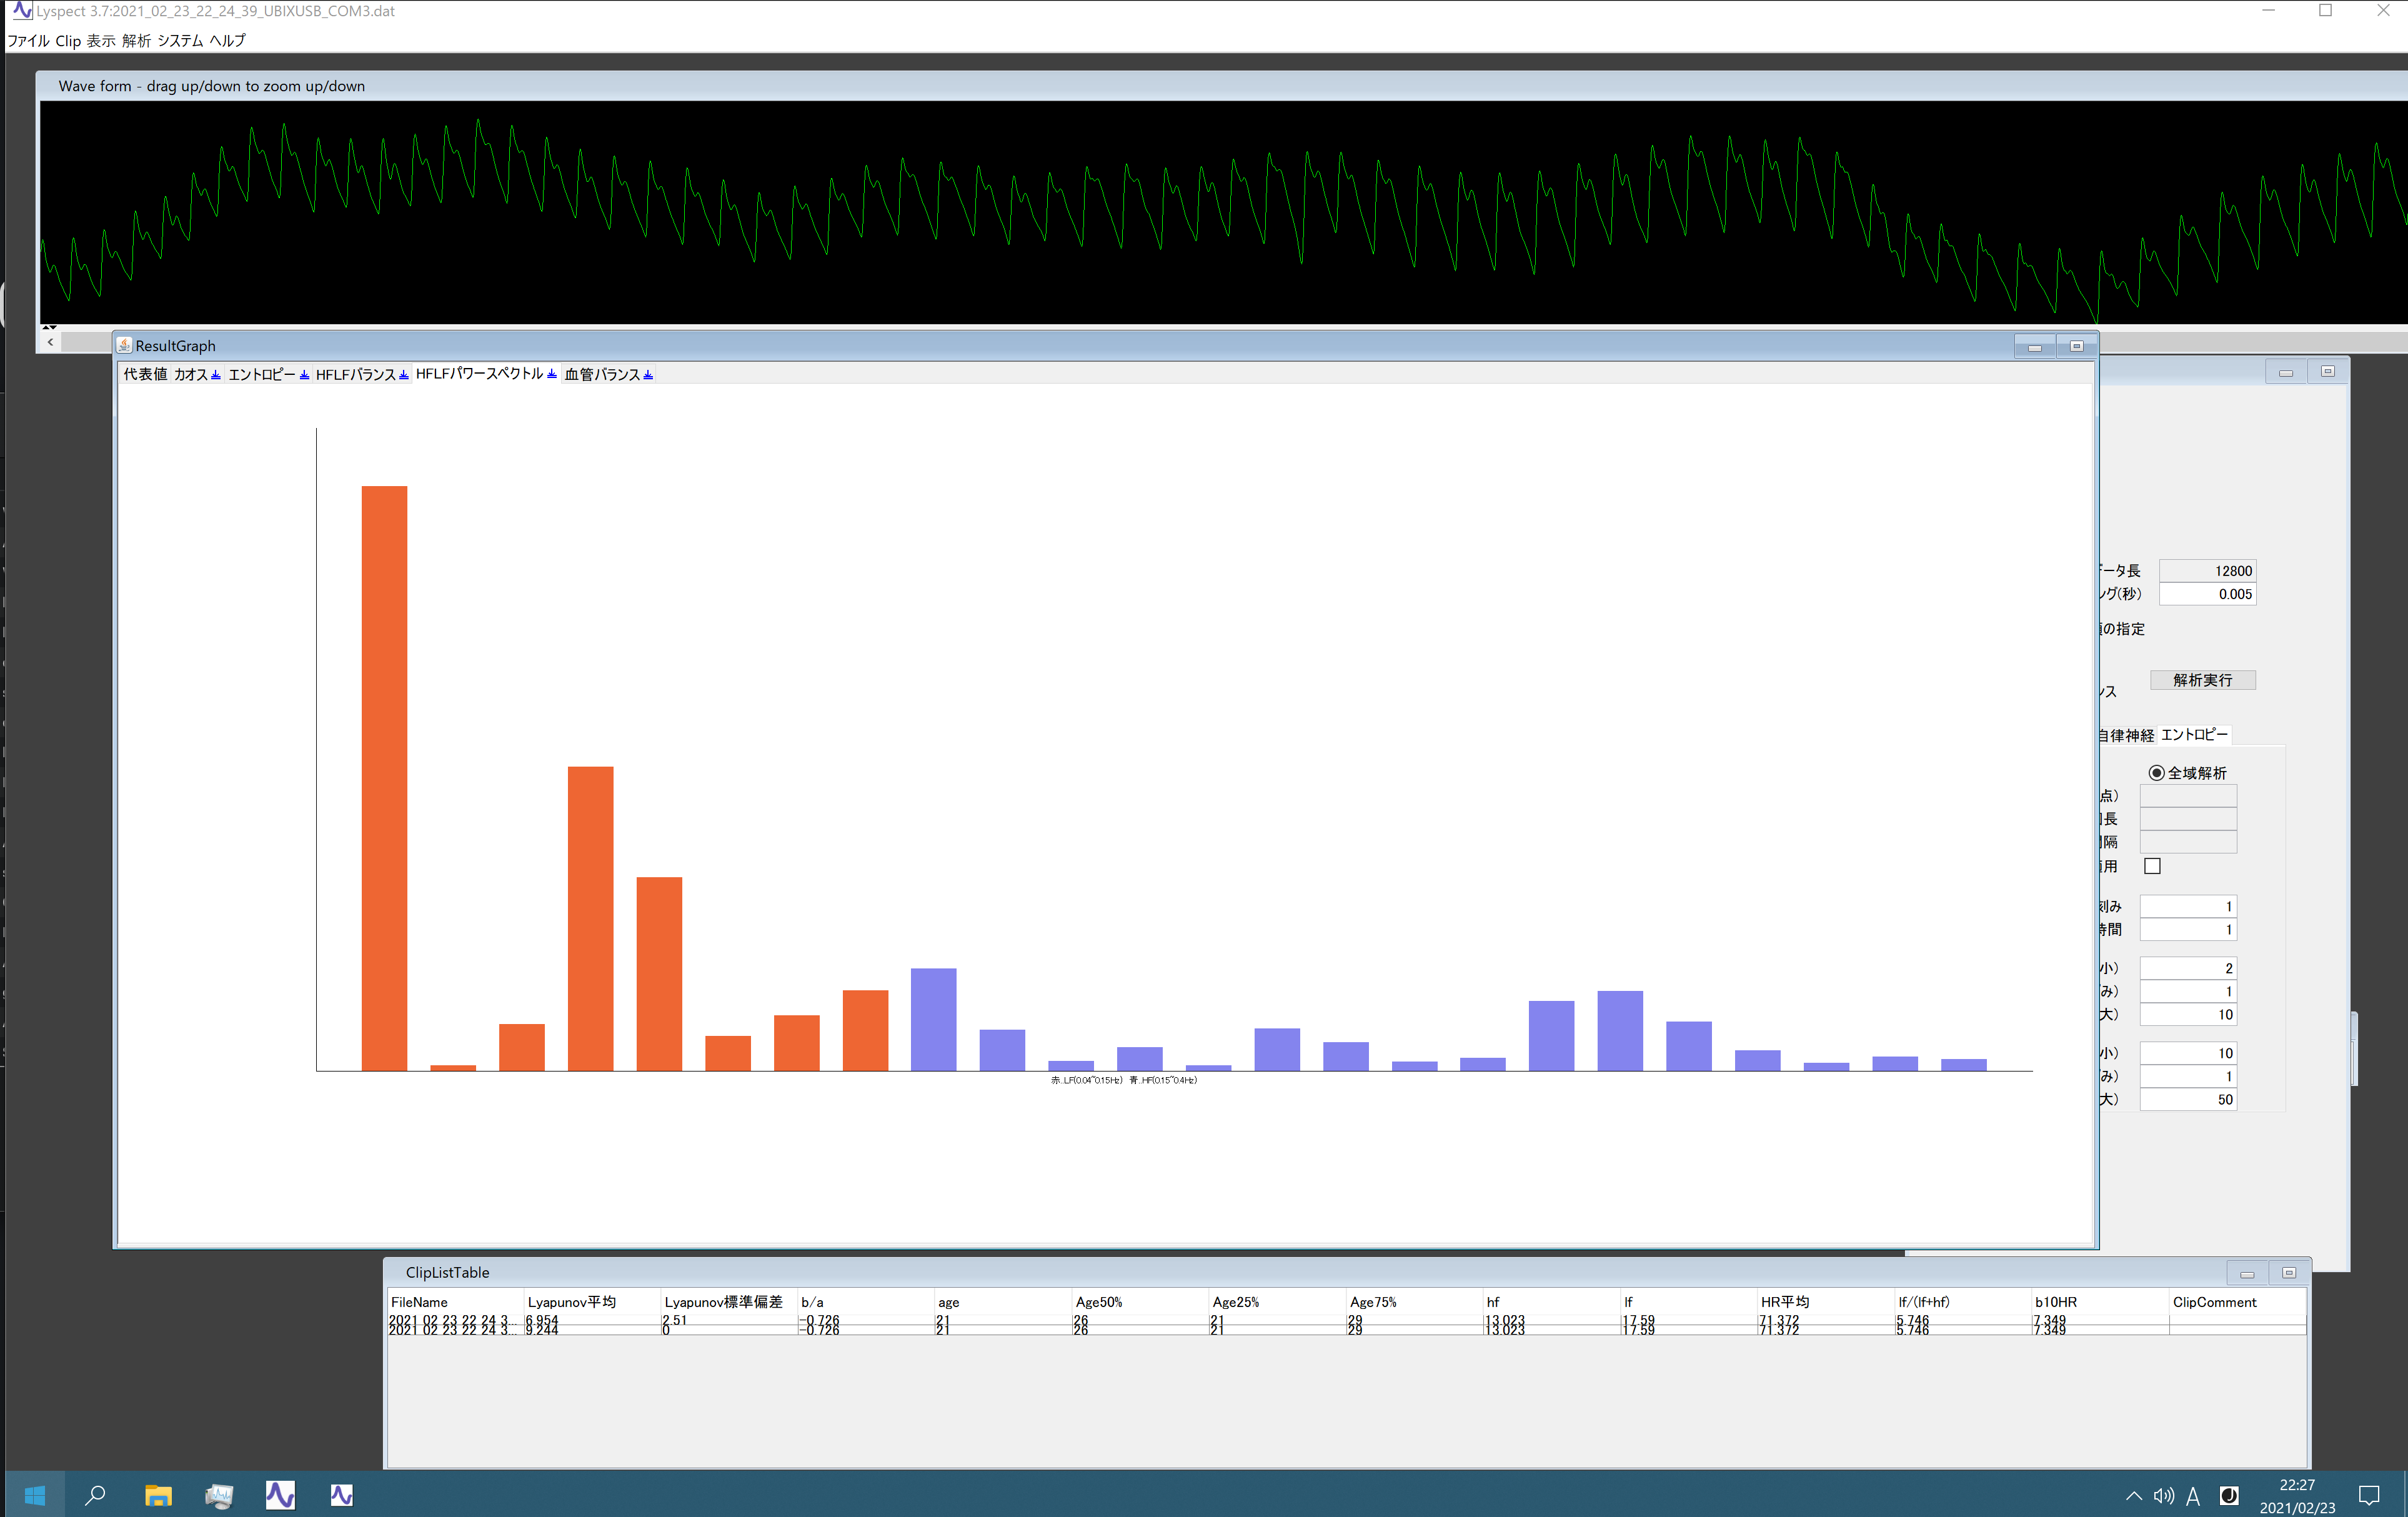
\includegraphics[width=100mm]{lyspect.png}}
    \end{center}
    \caption{Lyspectでの分析画面}
    \label{fig:lyspect}
  \end{minipage}
\end{figure}


\subsection{結果と考察}